%%%%%%%%%%%%%%%%%%%%%%%%%%%%%%%%%%%%%%%%%%%%%%%%%%%%%%%%%%%%%%%%%%%%%%%%%%%%%%
%
% Section file included in main project file using \input{}
%
% Assumes that LaTeX2e macros and packages defined in cg_comp.sty are
%   available
%
%%%%%%%%%%%%%%%%%%%%%%%%%%%%%%%%%%%%%%%%%%%%%%%%%%%%%%%%%%%%%%%%%%%%%%%%%%%%%%

 \section{Experimental Estimate of the String Constant\label{sct:exp}}

 \begin{figure}
  \centering
  \begin{subfigure}[b]{0.8\textwidth}
   \centering
   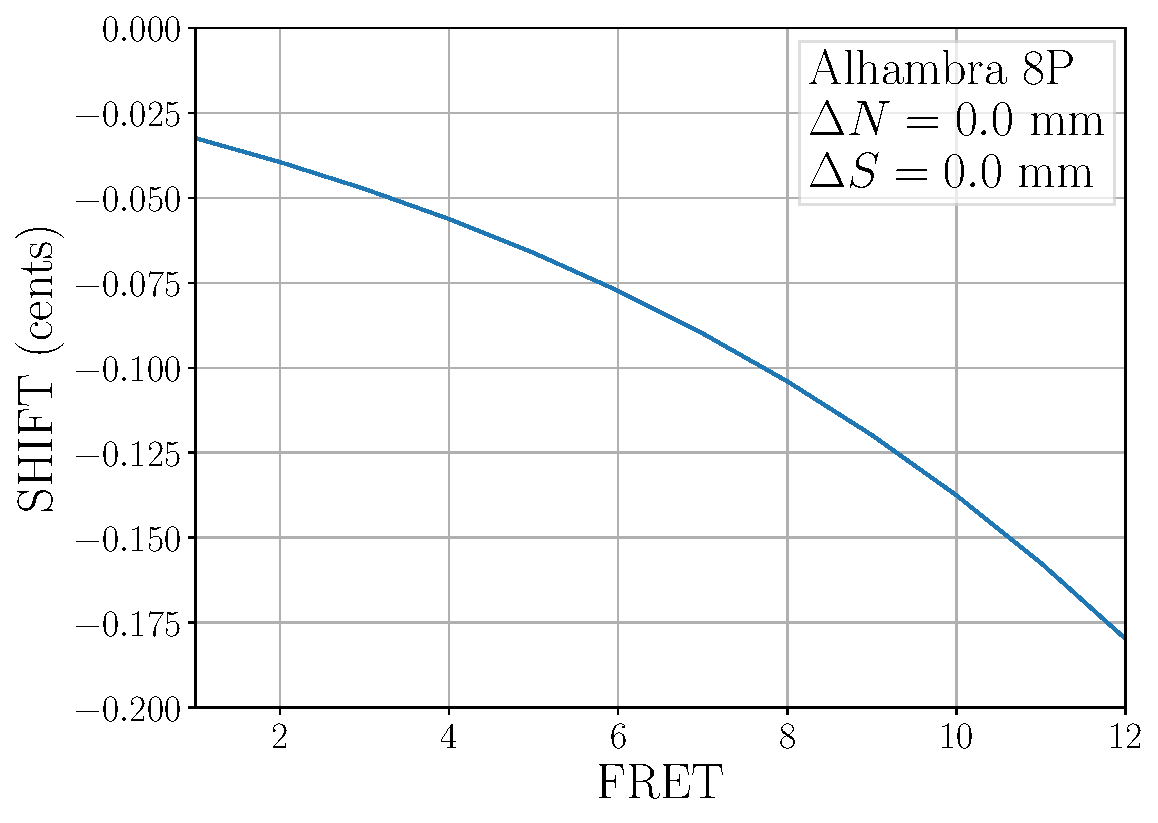
\includegraphics[width=5.0in]{figures/norm_error_uncompensated}
   \caption{Frequency shift for an uncompensated guitar}
   \label{fig:norm_error_uncompensated}
  \end{subfigure}
  \par\vspace{0.25in}
  \begin{subfigure}[b]{0.8\textwidth}
   \centering
   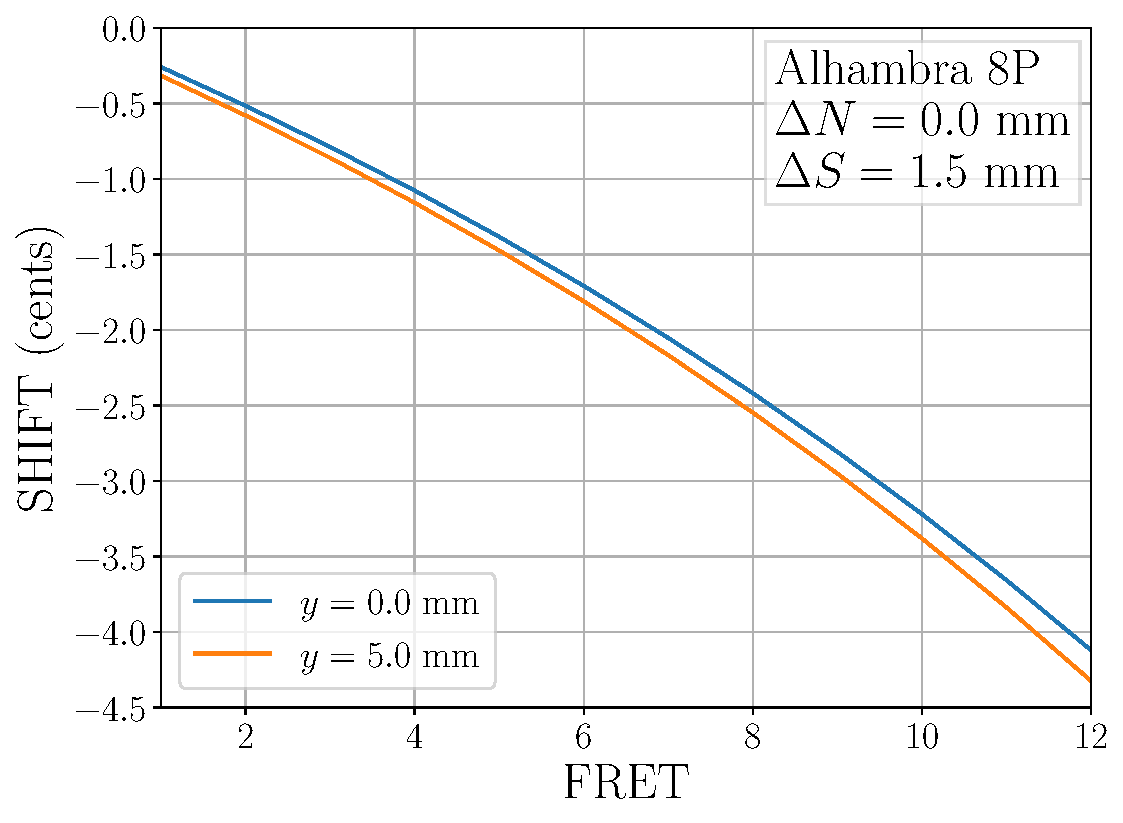
\includegraphics[width=5.0in]{figures/norm_error_factory}
   \caption{Frequency shift for a factory guitar}
   \label{fig:norm_error_factory}
  \end{subfigure}
  \caption{\label{fig:norm_error} Frequency shift (in cents) due to the fretted length $L_n$ for an uncompensated (a) and factory (b) Alhambra 8P guitar, for both zero and nonzero lateral displacement $y$.}
 \end{figure}

 \begin{figure}
  \centering
  \begin{subfigure}[b]{0.8\textwidth}
   \centering
   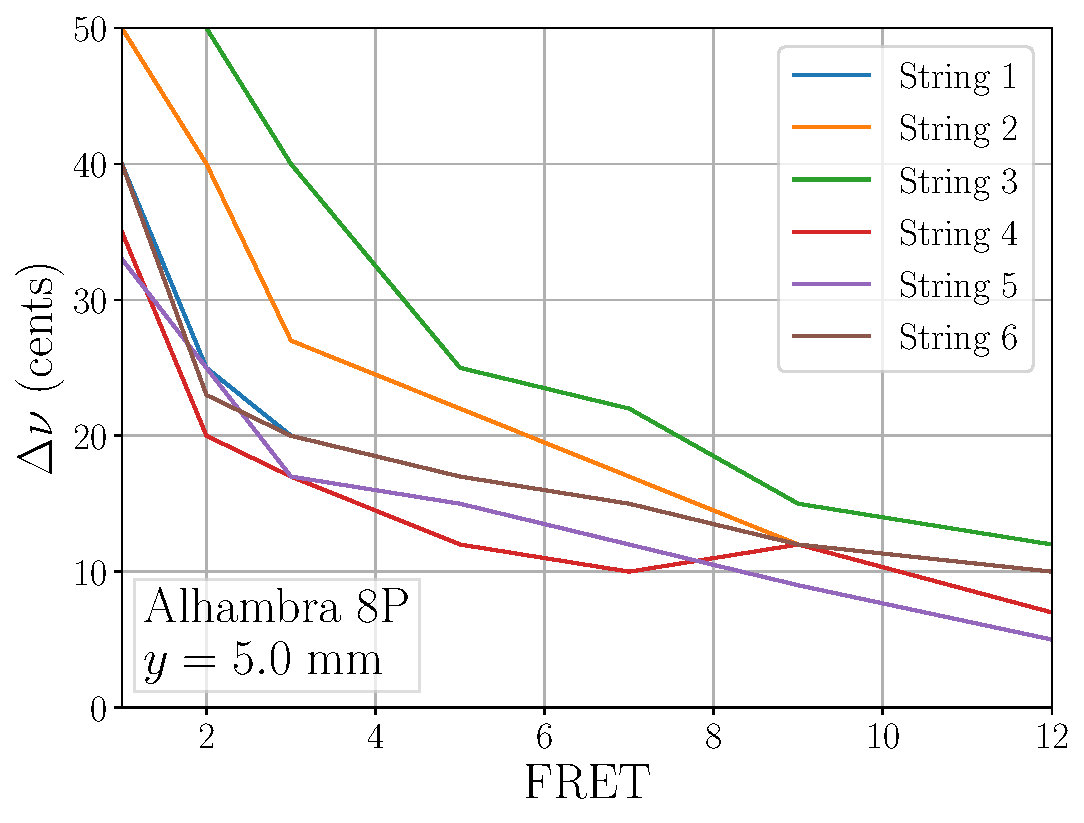
\includegraphics[width=5.0in]{figures/shift_data}
   \caption{Experimental data}
   \label{fig:shift_data}
  \end{subfigure}
  \par\vspace{0.25in}
  \begin{subfigure}[b]{0.8\textwidth}
   \centering
   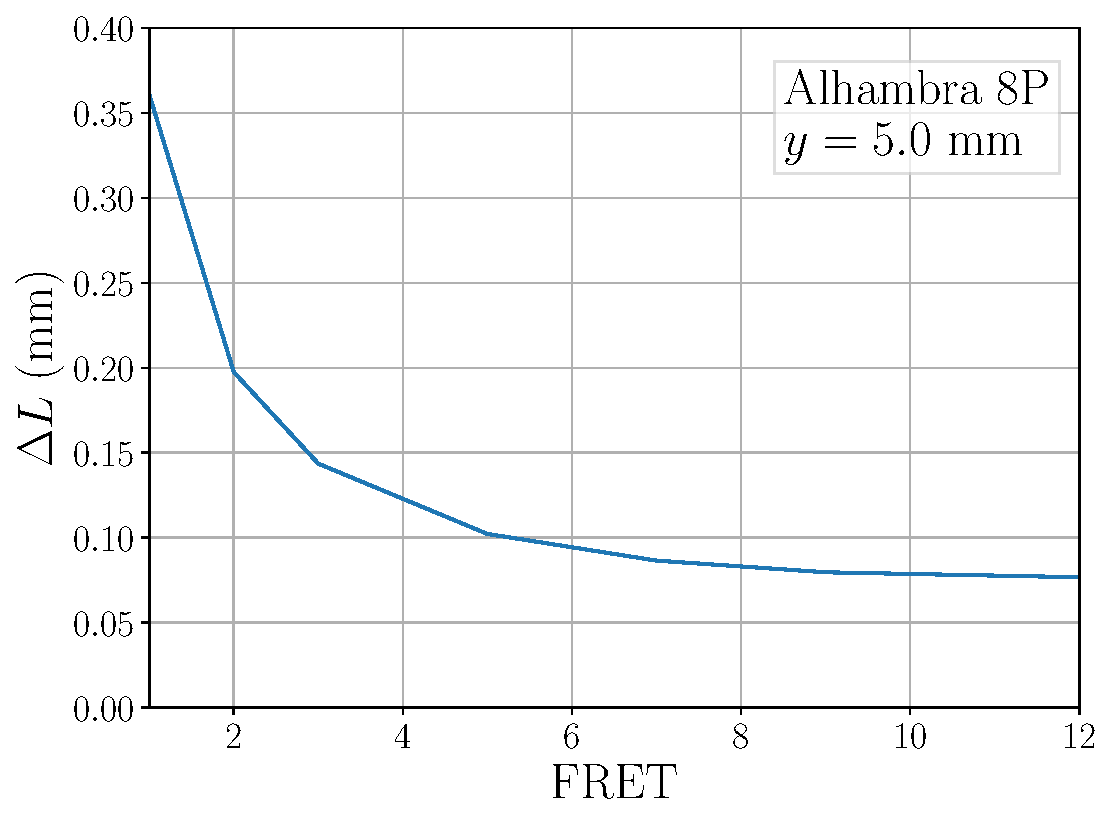
\includegraphics[width=5.0in]{figures/delta_l}
   \caption{Calculated change in total string length $\mathcal{L}$}
   \label{fig:delta_l}
  \end{subfigure}
  \caption{\label{fig:exp_data} Frequency shift (in cents) (a) and change in total string length $\mathcal{L}$ (b) due to lateral displacement $y$.}
 \end{figure}
